\head{Структуры данных, часть 3}
В прошлый раз мы познакомились с двумя деревьями: Деревом отрезков и Деревом Фенвика. На этом же уроке мы изучим ещё две древовидные структуры данных: кучу и декартово дерево. Куча является довольно специфичной структурой данных, так как она позволяет делать довольно мало операций, но взамен имеет маленькую скрытую асимптотику. Декартово дерево же можно рассматривать как мощную модификацию встроенных структур данных: массивов, множеств и куч.


\subhead{Куча}
\term{Куча (heap)} — полное двоичное дерево, в котором значение в вершине не меньше, чем значения во всех дочерних вершинах (так устроена \term{max-heap}, она же \term{невозрастающая куча} аналогично в \term{min-heap} (\term{неубывающей куче}) в вершине значение не больше, чем в дочерних). Полнота дерева означает, что все его слои заполняются последовательно, то есть новый слой добавляется только после того, как предыдущий полностью закончится.

\begin{wrapping}{0.34}
    Пример невозрастающей кучи можно увидеть на картинке справа. При этом оказывается, что кучу очень удобно хранить в массиве, ведь можно пронумеровать элементы кучи так же, как мы это делали в ДО. Тогда для вершины $p$ дочерними будут $2p$ и $2p + 1$, при этом нужно либо проверять, входят ли эти элементы в массив, или же дополнить его какими-то специальными значениями.
    \wrappedimg{0.55}{0.55}{max_heap.png}
\end{wrapping}

Куча должна поддерживать такие операции, как: добавление элемента, извлечение максимума (числа в корне) и удаление максимума. Дополнительно можно реализовать такие операции, как удаление произвольного элемента по индексу, слияние двух куч и смена приоритета элемента (тоже по индексу). Все эти операции можно реализовать через два типа \term{просеиваний}: вверх и вниз, которые будут работать за \O{\log n}, потому что на каждом шаге просеивания будут переходить на один уровень.

Чтобы добавить элемент, нам понадобится просеивание вверх: добавим наше число в конец кучи и после этого будем поднимать его наверх, пока свойство кучи будет нарушаться. Иными словами, мы будем обменивать местами родительскую вершину и дочернюю, если вдруг так оказалось, что они упорядочены неправильно. Понятно, что такое просеивание работает, ведь свойство кучи у нас нарушается максимум по одному ребру, с которым мы и работаем в текущий момент.

Просеивание вниз нам понадобится при удалении минимального значения. Удалять числа из начала массива — это затратная операция, поэтому мы сделаем так: обменяем первый и последний элемент местами, и удалим минимум (который теперь находится в конце). После этого нужно будет восстановить свойство кучи, для этого будем просеивать первый элемент вниз: если этот элемент портит кучу, то мы поменяем его с его наименьшим потомком. Так среди этих трёх вершин (элемента и двух дочерних) минимальное значение окажется родителем двух оставшихся, а значит наша куча стала чуть лучше.

Кроме того, просеивание вниз позволяет строить кучу за \O{n}, потому что можно запустить просеивания вниз от всех родительских вершин. А если запускать эти просеивания в обратном порядке (от $\lfloor\frac{n}{2}\rfloor$ до $1$), то оказывается, что получится линейное число операций (мы это доказывать не будем, но читатель может сделать это сам).

В коде это можно реализовать вот так:

% \cpp{ds-3}{55}
\nocode

Но видно, что кода получилось достаточно много, но это не беда, ведь в C++ есть встроенная куча, которая называется \lcpp{priority_queue}. Она, как и положено куче, позволяет добавлять элементы, получать максимальное значение и удалять его. Пример использования \term{очереди с приоритетом} есть ниже.

% \cpp{ds-3}{12}
\nocode

Стоит отметить, что в обеих реализациях значение в вершине является её приоритетом, но в общем случае, у каждой вершины отдельно может быть значение и приоритет. В таком случае нужно будем поменять тип, хранимые в вершине, например, на \lcpp{pair}.


\subhead{Декартово дерево}
\term{Декартово дерево} — это ещё одна древовидная структура данных, у которой есть и другие названия: \term{treap}, \term{дуча}, \term{дерамида} и \term{рандомизированное бинарное дерево поиска}. Формально, эта структура хранит в своих вершинах пары $(X, Y)$ так, что по $X$ она является бинарным деревом поиска, а по $Y$ — бинарной пирамидой (ничего не понятно, ведь?:)).

Но если посмотреть на картинку, то всё становится понятней. По $X$ (они ещё называются \term{ключами}) значения в левом поддереве меньше, чем в родительской вершине, а оно в свою очередь, меньше, чем в правом поддереве. По $Y$ же (другое название — \term{приоритет}) родительское значение больше, чем дочерние. Хоть Декарт и не придумывал эту структуру данных, но если расставить точки $(X, Y)$ на Декартовой плоскости, то мы как раз получим дерево.

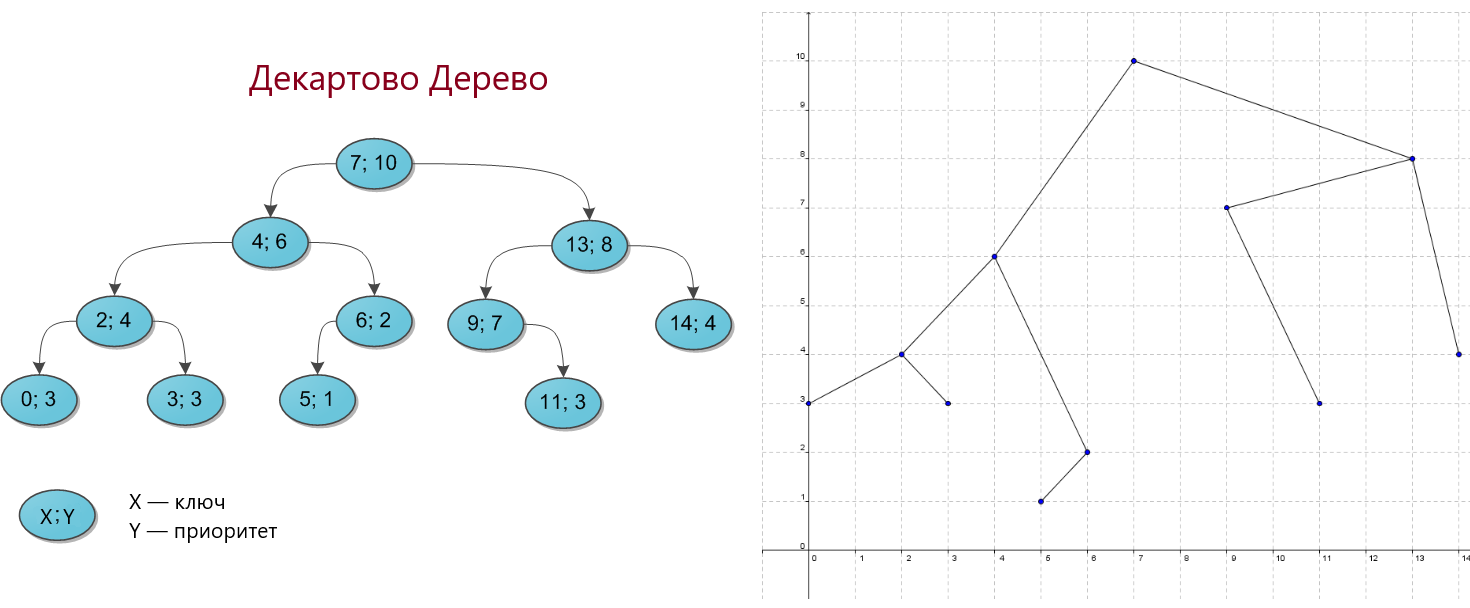
\includegraphics[scale=0.45]{img/treap.png}

Теперь перейдём к работе с Декартовым деревом (ДД), которое поддерживает достаточно много операций: добавление элементов, их поиск и удаление (по ключам). Кроме того, ДД может разбиваться на два других ДД по определённому ключу и также сопоставлять индексу элемента его значение и наоборот. Отсюда видно, что ДД объединяет в себе функционал массивов (получение элемента по индексу), множеств (поиск элементов) и куч (ДД является кучей по приоритетам), то есть такая структура может очень даже пригодиться.

При этом, так же, как и в куче, через две операции (разбиения и слияния) можно выразить все другие операции. Но перед этим стоит сказать, что в нашей реализации ДД в каждой вершине будут храниться: ключ, значение и \term{указатели} на левое и правое поддеревья. Про указатели нужно знать то, что это не сами данные, а лишь информация о месте их расположения. что позволит нам переходить от родительской вершины к дочерним. Кроме того, хранить всё ДД мы будем с помощью её корня.

Начнём с операции разбиения ДД по ключу $key$. Разбивать мы будем рекурсивно, начиная с корня, а получить мы хотим два ДД таких, что в левом все ключи меньше, чем $key$, а в правом — все остальные. Пусть мы сейчас находимся в какой-то вершинке и требуется разбить ДД, за которое она отвечает. Тогда по ключу в вершине мы можем понять, куда она пойдёт: 

\begin{itemize}
    \item Если ключ в вершине больше (или равен) $key$, то это значит, что вершина вместе со своим правым ребёнком должны оказаться в правом поддереве (так как по ключам у нас дерево поиска). То есть остаётся лишь рекурсивно разбить левую часть, и, очевидно, присоединить средний кусок из трёх к правому.
    \item Аналогично при ключе в вершине меньшим $key$ разбивать придётся правое поддерево. А из трёх образовавшихся частей две левых имеют ключи меньшие, чем $key$, поэтому из нужно объединить.
\end{itemize}

Операция слияния должна принимать два ДД и объединять их в одно. При этом у первого ДД все ключи должны быть меньше всех ключей второго ДД. А раз по ключам у нас всё определено, то остаётся лишь не нарушить приоритеты. Но здесь всё совсем просто: у одного из ДД в корне приоритет будет больше, чем у другого (пусть у первого, аналогично будет для второго), а поскольку в корне у нас самый большой приоритет, то после объединения корнем станет корень первого ДД. Но тогда мы точно знаем, что в левом поддереве ничего поменяться не может (из-за условия на ключи), а значит в правом поддереве нам нужно будет объединить правого сына первого ДД и второе ДД, что делается рекурсивно.

Две сложных операции мы разобрали, теперь остались операции попроще. Чтобы найти ключ, мы будем пользоваться отсортированностью ключей, и в зависимости от ключа в родителе, выбирать левого или правого сына. А для них поиск можно сделать рекурсивно.

Удаление элемента $key$ мы можем сделать через два разреза: сначала разрежем левее $key$ (в нашей реализации это разбиение по $key$), а после этого правую часть разделим правее $key$ (то есть сделаем разбиение по $key + 1$). Из полученных трёх частей в средней ключи равны $key$ и эту часть нужно удалить. Оставшиеся же части просто соединяем операцией слияния.

И последняя операция — это добавление. Во-первых, мы не хотим хранить повторяющиеся ключи, поэтому если добавляемый ключ уже есть, то ничего делать не будем. Иначе же, мы можем разрезать по этому ключу и объединить три ДД в одно: левое, сам элемент и правое.

Хоть описание получилось достаточно длинным, но в коде это выглядит коротко и лаконично.

% \cpp{ds-3}{54}
\nocode

Но реализация ДД — это хорошо, но ещё бы уметь её пользоваться. Поэтому приведём ещё и примеры работы с полученным ДД:

% \cpp{ds-3}{7}
\nocode

И ещё один нюанс — это функция \lcpp{random} в восьмой строке. Если приоритеты мы получаем из задачи, то эта функция нам не нужна, а если приоритетов нам никто не дал, то придётся генерировать их самостоятельно. За это и отвечает функция \lcpp{random}, которую нужно заменить на понравившийся способ генерировать случайные числа (о них написано в разделе \hyperlink{built-in function}{встроенные функции}).

Теперь немного поговорим, зачем нам нужна такая сложная структура данных, которая хранит кроме ключей ещё какие-то приоритеты. Если бы у нас не было приоритетов, то ключи должны были бы храниться в отсортированном порядке. Но если ключи бы добавлялись в отсортированном порядке, то вместо равномерной древовидной структуры получился бы \term{бамбук} (у каждой вершины. кроме последней, ровно один ребёнок). Тогда каждая операция с таким деревом поиска могла бы выполняться за \O{n}, что долго (потому что такая же сложность операций с массивом).

Но когда мы используем приоритеты, то получается сбалансированная структура, в которой количество уровней составляет \O{\log n}. Но ведь наши рекурсивные функции делают постоянное количество операций на одном уровне, а значит все они работают за \O{\log n}.

Но раньше было заявлено, что ДД — это очень мощная структура данных, а пока наше ДД умеет делать только операции, которые и так уже реализованы в \lcpp{set}. Но, это легко исправить, если научиться искать $k$-й элемент по ключам (или же по указателю на элемент получать его индекс). Этого не умеют обычные множества, но мы легко это можем добавить.

Для этого в каждой вершине будем дополнительно хранить количество вершин в её поддереве. Тогда чтобы узнать $k$-ый элемент мы пойдём от корня и сможем определять, в какую из дочерних вершин спуститься (как мы это делали в ДО). Аналогично узнаётся и индекс элемента. А чтобы размеры поддеревьев хранились правильно, достаточно в конце каждой функции, меняющие ДД, пересчитывать размеры поддерева. Таким образом мы сможем узнавать $k$-ый элемент за \O{\log n}.

Но и это ещё не всё, ведь существуют \term{неявные Декартовы деревья}. Неявные ДД — это ДД, которые хранят в себе массивы: приоритетом элемента является его значение, а ключом — индекс в массиве. Но ДД не зря называется неявным: мы не будем хранить ключи, потому что можем вычислять их во время спуска от корня. Вот так неожиданно получилось, что отказ от приоритетов вреден, а отказ от ключей полезен.

Чтобы вычислять ключи мы будем использовать уже описанную выше технику хранения размера поддеревьев. А поскольку индекс элемента в массиве равен количеству элементов, стоящих раньше искомого, то на каждом спуске к правому сыну мы будем прибавлять размер левого плюс один (размер родителя), а если будем спускаться к левому сыну, то добавлять ничего не будем.

Слияние в неявном ДД останется таким же, как и в явном (потому что там нигде не используются ключи). А вот функция разбиения теперь должна будет вычислять \lcpp{t -> key} перед её использованием согласно описанию выше: это размер левого поддерева плюс количество уже обработанных вершин (будем передавать его рекурсивно ещё одним параметром), или же просто размер левого поддерева, но тогда при переходе в правого сына нужно будет уменьшать $key$, который мы ищем (мы так уже делали в ДО). Таким же образом нужно обработать и \lcpp{t -> key} в функции поиска.

Поскольку мы определяли удаление и добавление элементов через слияния и разбиения, то наши производные функции продолжат работать. Поменяется лишь смысл $key$, которые они принимают: теперь это будет индекс, откуда нужно удалить или куда требуется вставить элемент.

Таким образом у нас получился аналог массива, который за \O{\log n} позволяет делать все операции с собой: добавление, поиск и удаление элементов. Но неявное ДД способно на большее.

Вспомним, что в ДО у нас было вычисление функций на диапазонах и их изменение. Оказывается, что и это умеет ДО, если будет хранить в себе дополнительную информацию.

Например, чтобы вычислить сумму на отрезке нам будет достаточно сохранить в каждой вершине сумму ей поддерева (эту сумму нужно обновлять, когда меняется поддерево). А когда для ответа на сам запрос, мы вырежем нужный кусок массива и в его корне будет храниться сумма на этом отрезке. После этого нужно не забыть восстановить ДД обратно.

А если нам потребует, например, прибавлять на отрезках. то мы дополнительно в вершинах будем хранить сумму прибавлений. Когда будет поступать запрос на обновление, то мы вырежем наш отрезок и в корне отрезка увеличим прибавление. После этого нам нужно будет вновь объединить все три части. Но теперь стоит немного поменять функции объединения и слияния, добавив в них проталкивание. Проталкивание мы запускаем от корневых вершин, меняем значение в корне и помечаем, что в дочерних вершинах нужно сделать обновления. А после этого операции слияния и объединения делаются без потери информации.

А теперь осознаем мощь ДД, пройдя операции, которое не умеет делать ДО. Во-первых, ДО не умеет себя разрезать на части и склеивать ДО из частей. А значит, что если нам, например, требуется сдвигать все элементы массива, то мы можем сделать это очень легко, с помощью стандартных операций ДД.

Также заметим, что ДД может даже разворачивать отрезки массива, если рассмотреть разворот, как операцию на изменения отрезка, а в момент проталкивания менять местами детей. Удивительная операция!

Вот мы и познакомились с ДД, которое умеет делать все операции массивов, множеств и ДО за \O{\log n}, а кроме того, умеет делать и специфичные операции. Также стоит сказать, что существует разреженное ДО, которое по своей сути напоминает неявное ДД.

